\section{Introduction}
\chapterauthor{Wiktor Czetyrbok, Kamil Dędza}
\par
Creating new products always begins with a clear idea, but even more importantly, with well-defined requirements. These requirements specify what needs to be done, by whom, by when, and with which resources. In the real estate field for example, according to International Journal of Real Estate and Land Planinng by Athanasios Lamprou and Dimitra Vagiona \cite{RealEstatePlanning},the most important criteria for the project success is time and budget, but it is also worth to mention that high up in the hierarchy is also business and commercial performance as well as technical
specifications and requirements. Both contribute to the importance of the requirements, and the same is within IT projects. In fact, over a half of the projects were challenged, meaning exceeded resources or lacking initially stated functionalities. Only 29\% are fully successful, whereas 19\% fail completely \cite{CriticalSuccessFactors}. 
\par
'Clarity is underappreciated as a requirements specification quality attribute. We studied the clarity of requirements forms, operationalized as ease of problem detection, least obstructive to understanding, and understandability by stakeholders' \cite{ClarityInRequirements}. Not only the process of gathering the requirements is critical, but also how they are stated. The language is not always straightforward, and not always provides the same meaning for every word. The understandability of the particular requirement is also a big concern. 
\par
One can ask, how to make the proper requirements? The first hint is to involve the customers and users during the requirements engineering process. It means that it is important to collaborate with the stakeholders and leads to 'better understanding of real needs' \cite{BestPractisesRE}. The other best practice is to ensure prioritization of the particular requirements. One way to achieve this is creating a field, where there is possibility to keep the level of importance of the particular tasks. One should not forget about allocating about 20\% of resources to the process of gathering the requirements \cite{BestPractisesRE}. This may feel like the resources are not efficiently allocated, but it will pay off in the future stages. 
\par
Having mentioned why requirements are not so straightforward for everyone, and what are the characteristics of accurate requirements, now the question arises what are the consequences of poorly gathered ones. Study from 2015 “Leading reasons for software project failure worldwide 2015” published by Statista Research Department \cite{FailuresStatisticaResearch} shows surprising results. The reason for almost half (48\%) of the failures are the changing or poorly documented requirements. This statistic underscores how a lack of clarity or shifting expectations can disrupt the entire project lifecycle, leading to misunderstandings, misaligned objectives, and ultimately, an end product that fails to meet user needs. Accurate requirements gathering is not merely a preliminary task but a critical phase that can define the project's success or failure. It is essential to invest the necessary time and resources upfront to capture a comprehensive, well-documented set of requirements to ensure alignment, efficiency, and a final product that truly meets stakeholder expectations. Requirements are the true, real foundation of the project. On the other side it is also worth mentioning that the second most popular reason is underfunding or under-resourcing and the third poor team or organizational management.

 \begin{figure}[H]
    \centering
    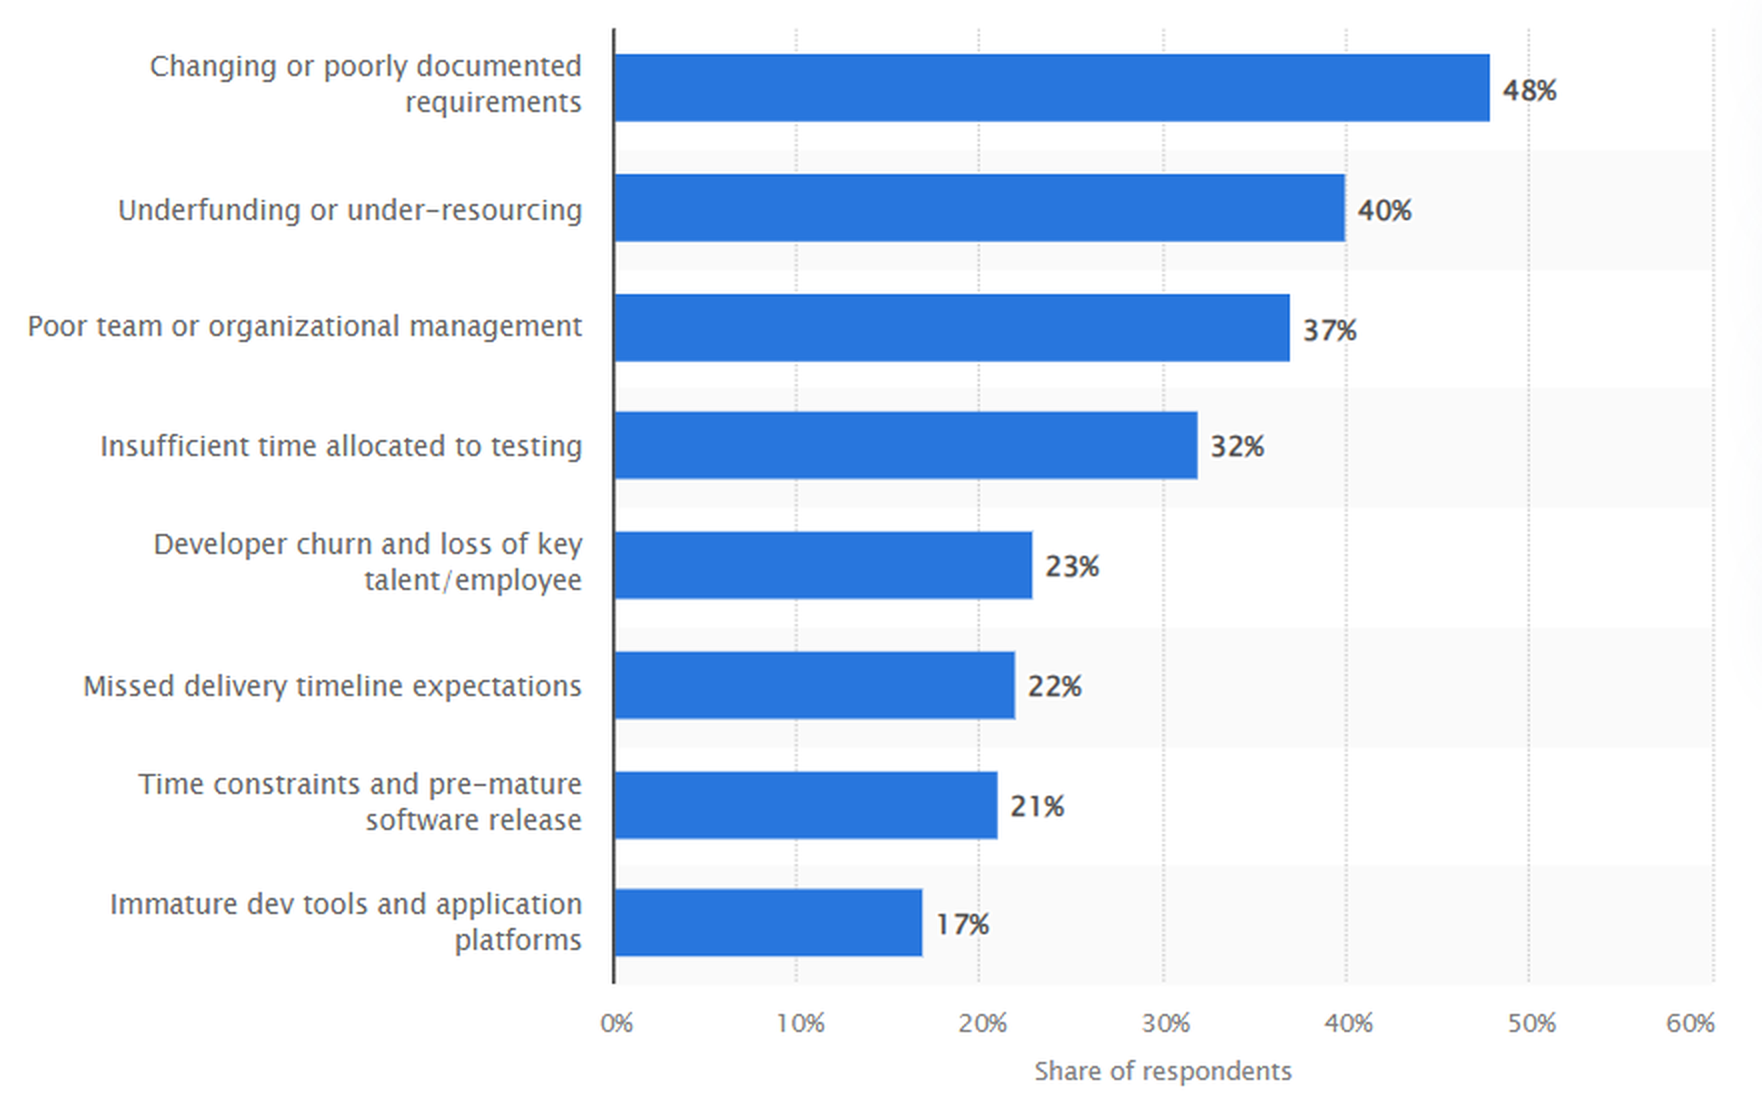
\includegraphics[width=1.15\textwidth]{images/statisticaresearch.png}
    \caption{ Leading reasons for software project failure \cite{FailuresStatisticaResearch}.}
    \label{xxx}
\end{figure}


\section{How to gather requirements}
\chapterauthor{Kamil Dędza}
\par
There are numerous techniques that are used during the process of gathering requirements. No single method suits all kinds of projects and is the golden rule that is used by every team. Each technique is tailored for uncovering specific information and suited for specific fields. For instance, a workshop, which is a meeting where many stakeholders, teams and experts can discuss and explore solutions, align on objectives and exchange ideas is facilitating the collaboration between all the parties. On the other hand there are interviews, where it is easy to dive deeper into the perspective of individuals and focus on their issue and their point of view. Observation is quite an interesting approach when it comes  to gathering requirements. The process relies on looking at the users and making notes about their problems and interactions. This method suits best real-life usage and uncovering implicit requirements. Document analysis is also common, especially when there are a lot of reports and for instance the availability of the stakeholder is limited. There are many more techniques other than those mentioned above \cite{MediumRequirementsAnalysis}, but even after listing all of them there would still not be one that is much better than the other ones. 'A combination of RE tools/techniques are more effective'\cite{CombineMethods}. Obviously, the mix of different techniques, when those that are chosen piece together, increases the likelihood of properly gathered requirements, hence also increases the likelihood of a solution that will be effective and suit the needs.
\par
During the development of the application personas were created. It is a user-oriented approach for gathering requirements, which focuses on the needs and issues. By creating the representatives of groups of future users it is easy to capture their diverse point of view. Each persona is a fictional character that has its own name, background, profession, problems and specific needs. It helps the developers to understand their situation by providing a human approach to the requirements. During requirements gathering, teams leverage these personas to evaluate how different users might approach the system, what functionalities are critical to each, and what workflows need prioritization to best serve diverse user needs. Often it is the case that the people responsible for creating the solution are biased, and do not see or understand other groups of users. Focusing on personas ensures that the designed system will in fact resolve real user challenges, taking into account different groups with different requirements. The three personas that have been created are described by the short description of their background - who they are, benefits - what advantages they can take by using the system, goals and challenges - what they want to achieve and what is preventing them, personality - their character, information technology skills - how they are able to interact with a system and fears - worries with regards to current situation without the existing solution. Each of these characteristics makes it much easier and more understandable to create the requirements for the system that they will use in the future. The representatives differ from one other by far, yet still they are to be using the system. To overcome this challenge of not creating three different solutions, it is crucial to understand the needs of every group and try to incorporate them into one, final system.
\begin{figure}[H]
    \centering
    \vspace{10pt} % Adds vertical space above
    \hspace{10pt} % Adds horizontal space (left)
    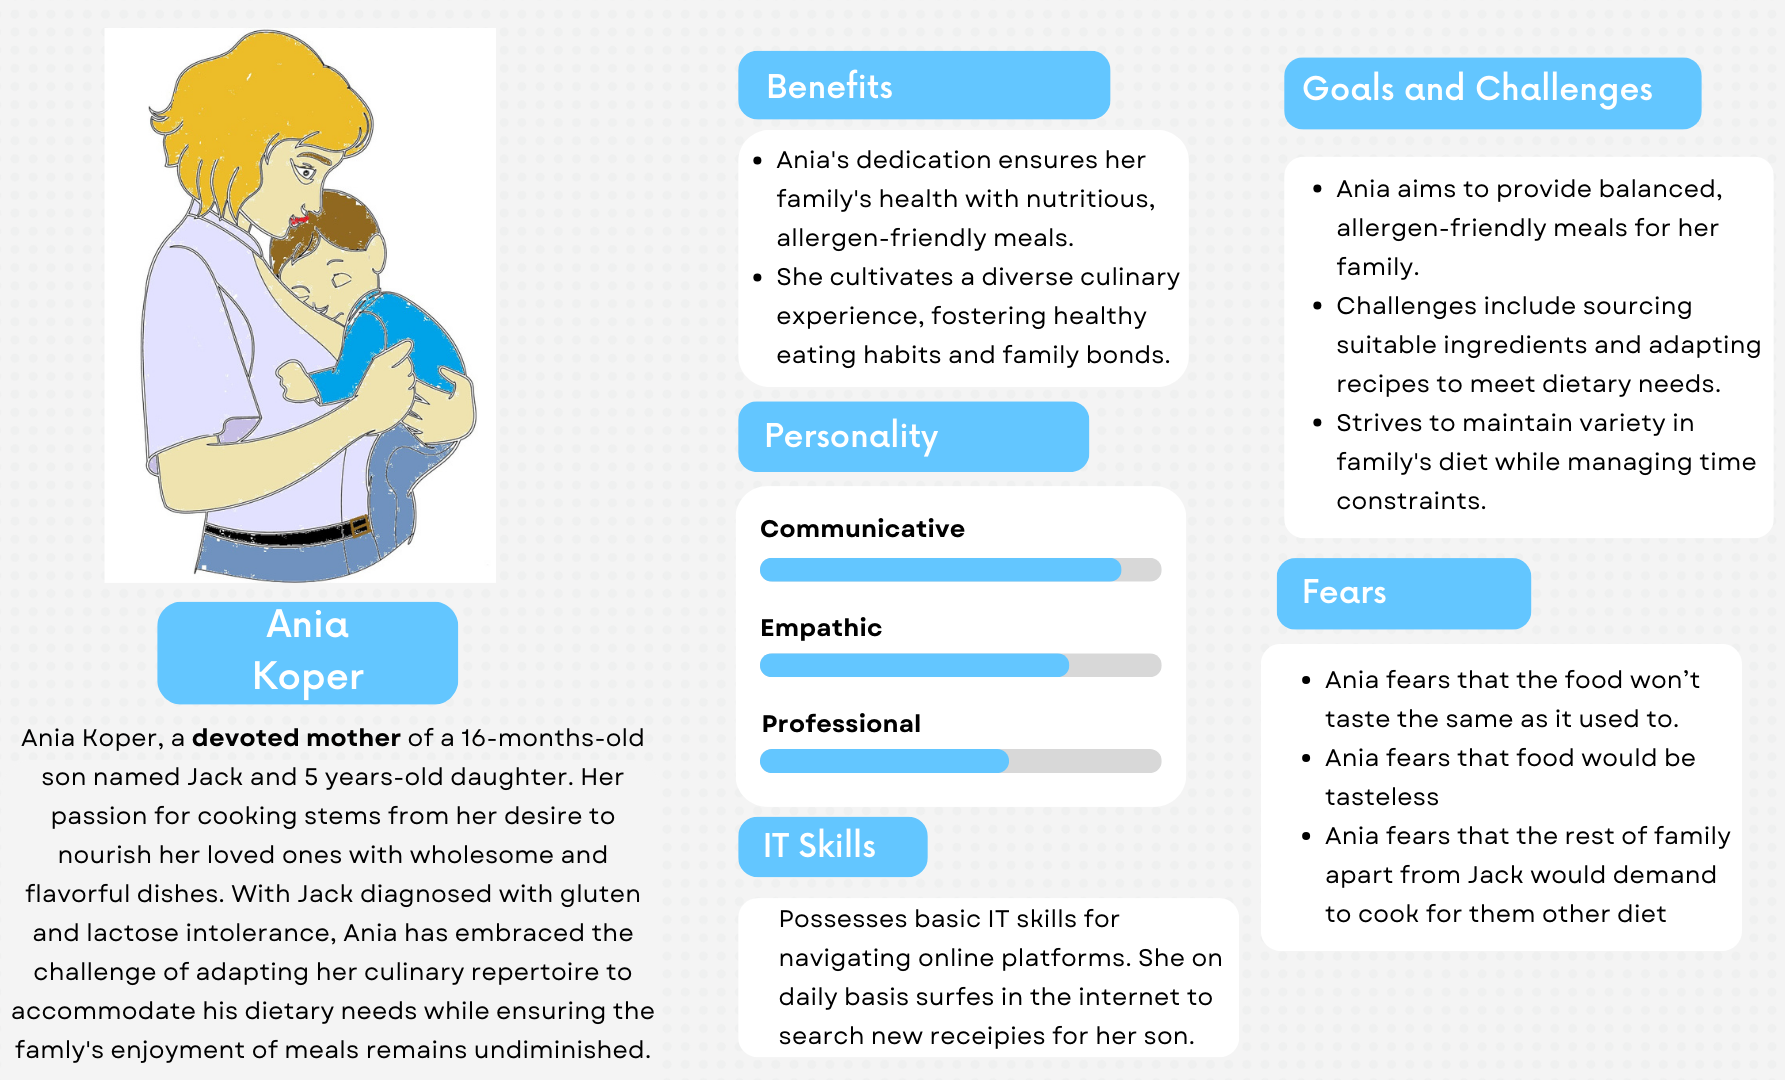
\includegraphics[width=1\textwidth]{images/Personas/1.png}
    \hspace{10pt} % Adds horizontal space (right)
    \vspace{10pt} % Adds vertical space below
    \caption{Persona 1}
    \label{xxx}
\end{figure}

\begin{figure}[H]
    \centering
    \hspace{5pt} % Adds horizontal space (left)
    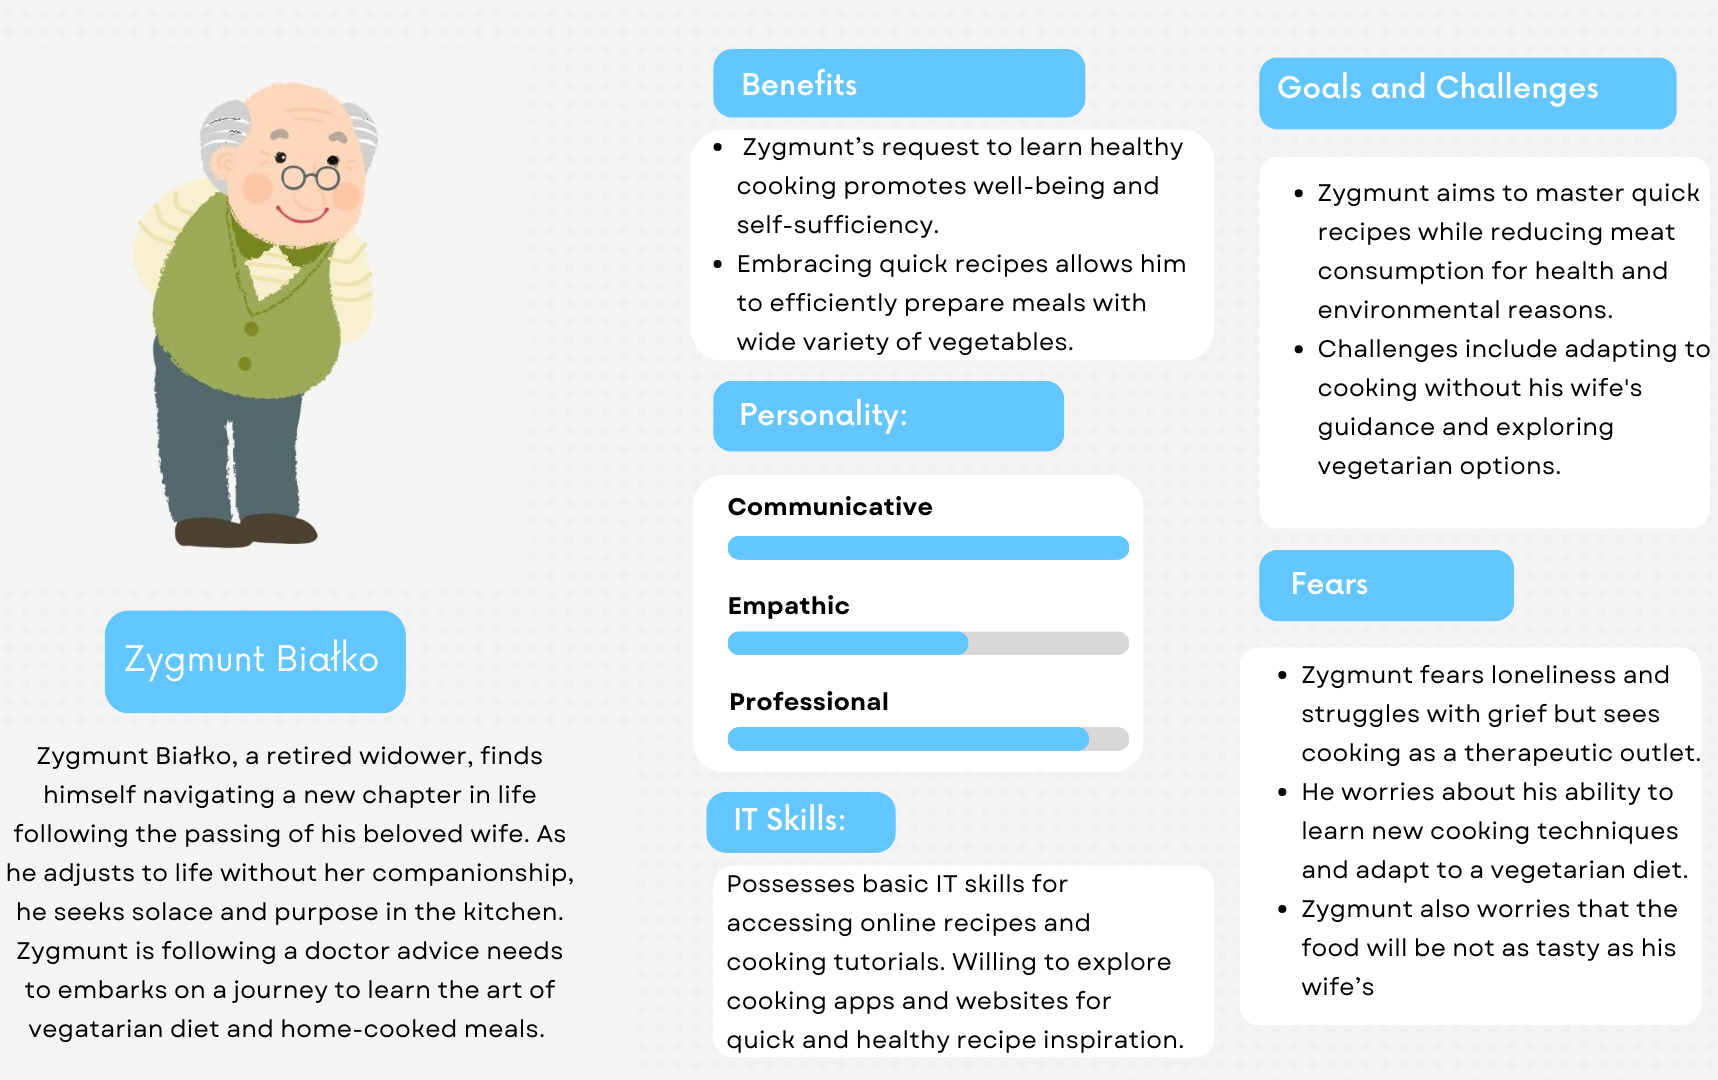
\includegraphics[width=1\textwidth]{images/Personas/2.png}
    \hspace{10pt} % Adds horizontal space (right)
    \vspace{10pt} % Adds vertical space below
    \caption{Persona 2}
    \label{xxx}
\end{figure}

\begin{figure}[H]
    \centering
    \hspace{5pt} % Adds horizontal space (left)
    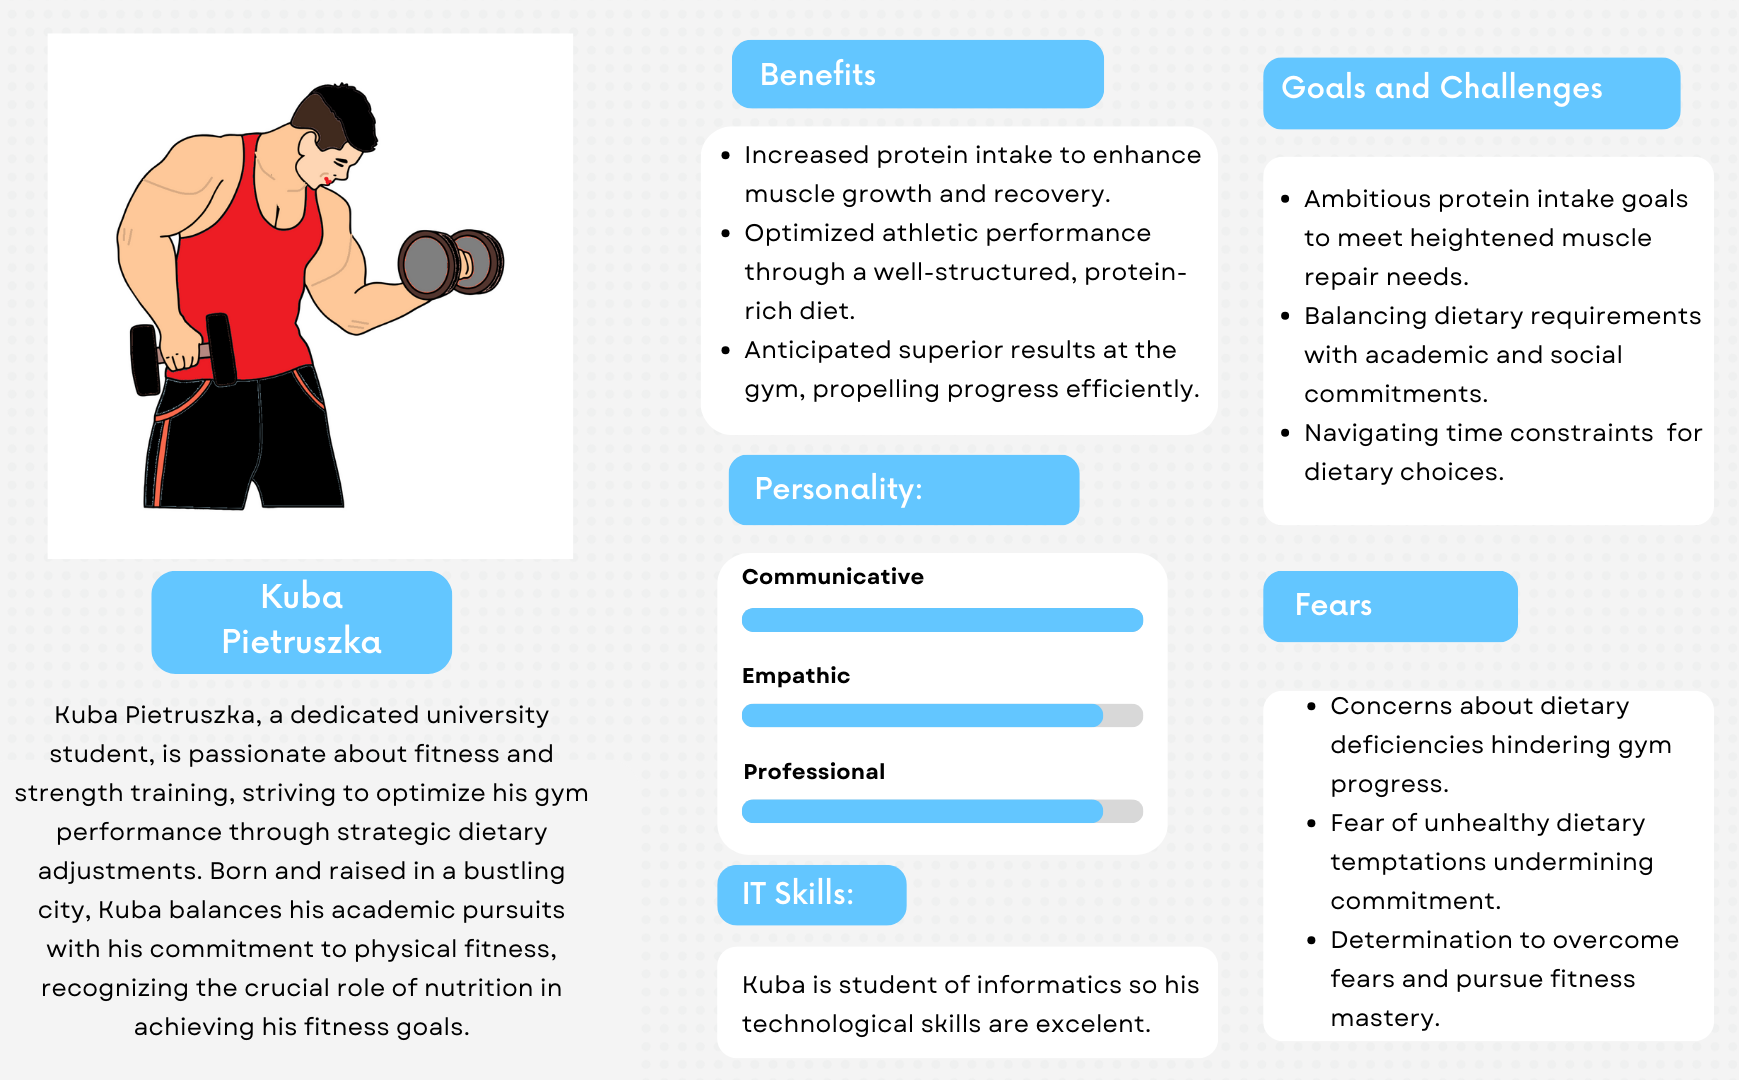
\includegraphics[width=1\textwidth]{images/Personas/3.png}
    \hspace{10pt} % Adds horizontal space (right)
    \vspace{10pt} % Adds vertical space below
    \caption{Persona 3}
    \label{xxx}
\end{figure}
\par		

'Most of the user story adopters (94 \%) use them in combination with Scrum' \cite{UserStories}, and is also a user-centered approach. The user stories are short, but the comprehensive descriptions can with ease capture the user needs in the form of a short story. The structure is simple, but yet provides valuable insights into the requirements. They start with who is the speaker, which could be the previously created personas, what he or she wants to achieve, and what are the benefits \cite{UserStories}. Each user story identifies the specific, unique action, linking it with an outcome. One of the key takeaways from utilizing this technique is that it helps with breaking complex problems into many smaller chunks in the form of a short, typically one sentence long story. The second advantage is that this approach also presents the benefit of specific action, so that the developers can understand why particular needs are so important and what benefits can the users take from them. By creating the user stories as part of the requirements developers can maintain a connection to the users’ needs. Last but not least, this method stimulates the iterative approach and prioritization of features that are actually strongly needed. There are many tools that support the creation of user stories, but Jira is the most popular and widely used. Everything is easily accessible by other team members, the stories can obviously have other fields apart from the description and name, but also the priority, assignee, estimate of work needed to accomplish, status, creation date just to name a few. These features keep the development organized, facilitate collaboration, and allow the team to adjust requirements flexibly throughout development, ensuring that the final product closely aligns with user expectations and agile principles.
\par
Prototyping is an iterative and interactive technique used during the process of gathering the requirements. 'Prototyping is the art of creating and evaluating a simple version of a product whose purpose it is to bring clarity on a specific topic' \cite{Prototype}. It is a low fidelity, preliminary version of the designed system. Its goal is to present some basic features or workflows, and let user stakeholders interact with the intermediate solution. Then the prototype can evolve and become an even more realistic version of the final product. The tangible version makes it extremely easier to be grasped by others, because it solves the problem of ambiguity of for example text. It is not the easiest task to describe some features, but the visual representation is much more effortless. By interaction with the prototype, developers are able to detect the issues with the workflows. Quick feedback is what characterizes this approach. Low quality sketches or drawings presented to the stakeholders can immediately clarify the ideas and enhance interaction. This technique is great when it comes to solving the misunderstanding, because it provides a clear vision of what the goal is, and how the product is likely to look in the future stages. Market is full of tools ready to help with creating the prototypes. One of the most popular is Figma. It provides the features for clickable mockups and many more interactive elements, enhancing the quality of collaboration with the stakeholders. 



